\documentclass[11pt]{article}
\usepackage[a4paper,margin=2.3cm]{geometry}
\usepackage{graphicx}
\usepackage{booktabs}
\usepackage{amsmath}
\usepackage[numbers,sort&compress]{natbib}
\usepackage[hidelinks]{hyperref}
\usepackage{xcolor}
% GENERATED by python/build_manuscript_inputs.py - do not edit
\newcommand{\AbaRatio}{0.30}
\newcommand{\AphCotOpen}{72.3}
\newcommand{\AphCotOut}{63.3}
\newcommand{\AphER}{31.4}
\newcommand{\AphEthHs}{0.0}
\newcommand{\AphEthInt}{33.7}
\newcommand{\AphHook}{21}
\newcommand{\AphHyp}{2591}
\newcommand{\AphHypoFrac}{22}
\newcommand{\AphOCore}{0.00}
\newcommand{\AphOSurf}{13.02}
\newcommand{\AphRoot}{3813}
\newcommand{\AphRootAngle}{180}
\newcommand{\AphSh}{3.41}
\newcommand{\AphTR}{23.8}
\newcommand{\BricCotOpen}{n.a.}
\newcommand{\BricCotOut}{52.1}
\newcommand{\BricER}{29.1}
\newcommand{\BricEthHs}{84.2}
\newcommand{\BricEthInt}{125}
\newcommand{\BricExploCotOpen}{n.a.}
\newcommand{\BricExploCotOut}{53.2}
\newcommand{\BricExploER}{30.3}
\newcommand{\BricExploEthHs}{143}
\newcommand{\BricExploEthInt}{223}
\newcommand{\BricExploHook}{184}
\newcommand{\BricExploHyp}{7743}
\newcommand{\BricExploHypoFrac}{23}
\newcommand{\BricExploOCore}{0.00}
\newcommand{\BricExploOSurf}{10.00}
\newcommand{\BricExploRoot}{2387}
\newcommand{\BricExploRootAngle}{180}
\newcommand{\BricExploSh}{2.00}
\newcommand{\BricExploTR}{22.5}
\newcommand{\BricHook}{185}
\newcommand{\BricHsEnd}{18.4}
\newcommand{\BricHsStart}{21.2}
\newcommand{\BricHyp}{7174}
\newcommand{\BricHypoFrac}{21}
\newcommand{\BricLedCotOpen}{63.2}
\newcommand{\BricLedCotOut}{62.3}
\newcommand{\BricLedER}{28.9}
\newcommand{\BricLedEthHs}{51.1}
\newcommand{\BricLedEthInt}{68.1}
\newcommand{\BricLedHook}{45}
\newcommand{\BricLedHyp}{2436}
\newcommand{\BricLedHypoFrac}{21}
\newcommand{\BricLedOCore}{0.00}
\newcommand{\BricLedOSurf}{13.21}
\newcommand{\BricLedRoot}{3281}
\newcommand{\BricLedRootAngle}{180}
\newcommand{\BricLedSh}{2.00}
\newcommand{\BricLedTR}{21.0}
\newcommand{\BricOCore}{0.00}
\newcommand{\BricOSurf}{11.91}
\newcommand{\BricOneGCotOpen}{n.a.}
\newcommand{\BricOneGCotOut}{55.3}
\newcommand{\BricOneGER}{32.3}
\newcommand{\BricOneGEthHs}{76.5}
\newcommand{\BricOneGEthInt}{120}
\newcommand{\BricOneGHook}{184}
\newcommand{\BricOneGHyp}{7144}
\newcommand{\BricOneGHypoFrac}{21}
\newcommand{\BricOneGOCore}{0.00}
\newcommand{\BricOneGOSurf}{11.91}
\newcommand{\BricOneGRoot}{2230}
\newcommand{\BricOneGRootAngle}{270}
\newcommand{\BricOneGSh}{2.00}
\newcommand{\BricOneGTR}{24.4}
\newcommand{\BricRoot}{2258}
\newcommand{\BricRootAngle}{180}
\newcommand{\BricSh}{2.00}
\newcommand{\BricTR}{21.3}
\newcommand{\CaraCotOpen}{64.3}
\newcommand{\CaraCotOut}{63.4}
\newcommand{\CaraER}{28.8}
\newcommand{\CaraEthHs}{0.5}
\newcommand{\CaraEthInt}{32.6}
\newcommand{\CaraHook}{19}
\newcommand{\CaraHyp}{2357}
\newcommand{\CaraHypoFrac}{20}
\newcommand{\CaraOCore}{0.00}
\newcommand{\CaraOSurf}{13.36}
\newcommand{\CaraRoot}{3623}
\newcommand{\CaraRootAngle}{180}
\newcommand{\CaraSh}{2.00}
\newcommand{\CaraTR}{20.9}
\newcommand{\CounterCotOpen}{86.4}
\newcommand{\CounterCotOut}{85.5}
\newcommand{\CounterER}{49.9}
\newcommand{\CounterEthHs}{1.8}
\newcommand{\CounterEthInt}{42.1}
\newcommand{\CounterHook}{17}
\newcommand{\CounterHyp}{1296}
\newcommand{\CounterHypoFrac}{38}
\newcommand{\CounterOCore}{0.00}
\newcommand{\CounterOSurf}{6.97}
\newcommand{\CounterRoot}{1658}
\newcommand{\CounterRootAngle}{270}
\newcommand{\CounterSh}{2.00}
\newcommand{\CounterTR}{38.7}
\newcommand{\EmcsLunarCotOpen}{58.1}
\newcommand{\EmcsLunarCotOut}{57.1}
\newcommand{\EmcsLunarER}{25.8}
\newcommand{\EmcsLunarEthHs}{0.0}
\newcommand{\EmcsLunarEthInt}{36.9}
\newcommand{\EmcsLunarHook}{19}
\newcommand{\EmcsLunarHyp}{2805}
\newcommand{\EmcsLunarHypoFrac}{23}
\newcommand{\EmcsLunarOCore}{0.00}
\newcommand{\EmcsLunarOSurf}{12.44}
\newcommand{\EmcsLunarRoot}{4166}
\newcommand{\EmcsLunarRootAngle}{270}
\newcommand{\EmcsLunarSh}{2.26}
\newcommand{\EmcsLunarTR}{18.9}
\newcommand{\EmcsMarsCotOpen}{58.5}
\newcommand{\EmcsMarsCotOut}{57.6}
\newcommand{\EmcsMarsER}{26.3}
\newcommand{\EmcsMarsEthHs}{0.0}
\newcommand{\EmcsMarsEthInt}{36.8}
\newcommand{\EmcsMarsHook}{19}
\newcommand{\EmcsMarsHyp}{2805}
\newcommand{\EmcsMarsHypoFrac}{23}
\newcommand{\EmcsMarsOCore}{0.00}
\newcommand{\EmcsMarsOSurf}{12.70}
\newcommand{\EmcsMarsRoot}{4101}
\newcommand{\EmcsMarsRootAngle}{270}
\newcommand{\EmcsMarsSh}{2.26}
\newcommand{\EmcsMarsTR}{19.4}
\newcommand{\EmcsOneCotOpen}{58.9}
\newcommand{\EmcsOneCotOut}{57.9}
\newcommand{\EmcsOneER}{26.8}
\newcommand{\EmcsOneEthHs}{0.0}
\newcommand{\EmcsOneEthInt}{36.7}
\newcommand{\EmcsOneHook}{18}
\newcommand{\EmcsOneHyp}{2807}
\newcommand{\EmcsOneHypoFrac}{23}
\newcommand{\EmcsOneOCore}{0.00}
\newcommand{\EmcsOneOSurf}{12.74}
\newcommand{\EmcsOneRoot}{4092}
\newcommand{\EmcsOneRootAngle}{270}
\newcommand{\EmcsOneSh}{2.26}
\newcommand{\EmcsOneTR}{19.8}
\newcommand{\EmcsZeroCotOpen}{56.6}
\newcommand{\EmcsZeroCotOut}{55.7}
\newcommand{\EmcsZeroER}{24.1}
\newcommand{\EmcsZeroEthHs}{0.0}
\newcommand{\EmcsZeroEthInt}{36.6}
\newcommand{\EmcsZeroHook}{21}
\newcommand{\EmcsZeroHyp}{2796}
\newcommand{\EmcsZeroHypoFrac}{23}
\newcommand{\EmcsZeroOCore}{0.00}
\newcommand{\EmcsZeroOSurf}{12.28}
\newcommand{\EmcsZeroRoot}{4202}
\newcommand{\EmcsZeroRootAngle}{180}
\newcommand{\EmcsZeroSh}{2.26}
\newcommand{\EmcsZeroTR}{17.3}
\newcommand{\EthTenCotOpen}{n.a.}
\newcommand{\EthTenCotOut}{88.1}
\newcommand{\EthTenER}{28.5}
\newcommand{\EthTenEthHs}{10000}
\newcommand{\EthTenEthInt}{10036}
\newcommand{\EthTenHook}{260}
\newcommand{\EthTenHyp}{805}
\newcommand{\EthTenHypoFrac}{20}
\newcommand{\EthTenOCore}{0.00}
\newcommand{\EthTenOSurf}{13.05}
\newcommand{\EthTenRoot}{601}
\newcommand{\EthTenRootAngle}{270}
\newcommand{\EthTenSh}{2.00}
\newcommand{\EthTenTR}{23.6}
\newcommand{\ExploCotOpen}{73.0}
\newcommand{\ExploCotOut}{66.1}
\newcommand{\ExploER}{33.5}
\newcommand{\ExploEthHs}{4.6}
\newcommand{\ExploEthInt}{56.5}
\newcommand{\ExploHook}{47}
\newcommand{\ExploHyp}{2219}
\newcommand{\ExploHypoFrac}{22}
\newcommand{\ExploOCore}{0.00}
\newcommand{\ExploOSurf}{11.65}
\newcommand{\ExploRoot}{3221}
\newcommand{\ExploRootAngle}{270}
\newcommand{\ExploSh}{2.00}
\newcommand{\ExploTR}{25.4}
\newcommand{\FitCap}{0.60}
\newcommand{\FitER}{32.0}
\newcommand{\FitLoss}{0.44}
\newcommand{\FitNFree}{9}
\newcommand{\FitNTargets}{6}
\newcommand{\FitOnset}{19.0}
\newcommand{\FitPeak}{7}
\newcommand{\FitTR}{24.0}
\newcommand{\GbcCotOpen}{n.a.}
\newcommand{\GbcCotOut}{53.5}
\newcommand{\GbcER}{30.5}
\newcommand{\GbcEthHs}{0.0}
\newcommand{\GbcEthInt}{46.7}
\newcommand{\GbcHook}{180}
\newcommand{\GbcHyp}{7599}
\newcommand{\GbcHypoFrac}{20}
\newcommand{\GbcMassHigh}{0.99}
\newcommand{\GbcMassLow}{0.95}
\newcommand{\GbcMassMid}{0.96}
\newcommand{\GbcOCore}{0.00}
\newcommand{\GbcOSurf}{13.34}
\newcommand{\GbcRoot}{2366}
\newcommand{\GbcRootAngle}{270}
\newcommand{\GbcSh}{2.02}
\newcommand{\GbcTR}{22.4}
\newcommand{\GbcUHigh}{0.116}
\newcommand{\GbcULow}{0.053}
\newcommand{\GbcUMid}{0.088}
\newcommand{\GroundCotOpen}{73.0}
\newcommand{\GroundCotOut}{65.3}
\newcommand{\GroundDarkCotOpen}{n.a.}
\newcommand{\GroundDarkCotOut}{55.0}
\newcommand{\GroundDarkER}{32.0}
\newcommand{\GroundDarkEthHs}{4.7}
\newcommand{\GroundDarkEthInt}{51.6}
\newcommand{\GroundDarkHook}{180}
\newcommand{\GroundDarkHyp}{7512}
\newcommand{\GroundDarkHypoFrac}{20}
\newcommand{\GroundDarkOCore}{0.00}
\newcommand{\GroundDarkOSurf}{13.38}
\newcommand{\GroundDarkRoot}{2335}
\newcommand{\GroundDarkRootAngle}{270}
\newcommand{\GroundDarkSh}{2.00}
\newcommand{\GroundDarkTR}{24.0}
\newcommand{\GroundER}{32.0}
\newcommand{\GroundEthHs}{2.8}
\newcommand{\GroundEthInt}{33.1}
\newcommand{\GroundHook}{30}
\newcommand{\GroundHyp}{2266}
\newcommand{\GroundHypoFrac}{20}
\newcommand{\GroundOCore}{0.00}
\newcommand{\GroundOSurf}{13.48}
\newcommand{\GroundRoot}{3369}
\newcommand{\GroundRootAngle}{270}
\newcommand{\GroundSh}{2.00}
\newcommand{\GroundTR}{24.0}
\newcommand{\HydEightyFiveModel}{none by 200}
\newcommand{\HydEightyFiveTheory}{81.4}
\newcommand{\HydFiftyFiveModel}{none by 200}
\newcommand{\HydFiftyFiveTheory}{47.6}
\newcommand{\HydFortyModel}{83.5}
\newcommand{\HydFortyTheory}{39.4}
\newcommand{\HydQuarterModel}{52.1}
\newcommand{\HydQuarterTheory}{33.6}
\newcommand{\HydZeroModel}{32.0}
\newcommand{\HydZeroTheory}{27.0}
\newcommand{\HypoFiveCotOpen}{n.a.}
\newcommand{\HypoFiveCotOut}{n.a.}
\newcommand{\HypoFiveER}{63.7}
\newcommand{\HypoFiveEthHs}{0.1}
\newcommand{\HypoFiveEthInt}{11.9}
\newcommand{\HypoFiveHook}{95}
\newcommand{\HypoFiveHyp}{286}
\newcommand{\HypoFiveHypoFrac}{53}
\newcommand{\HypoFiveOCore}{0.00}
\newcommand{\HypoFiveOSurf}{3.07}
\newcommand{\HypoFiveRoot}{177}
\newcommand{\HypoFiveRootAngle}{247}
\newcommand{\HypoFiveSh}{2.00}
\newcommand{\HypoFiveTR}{51.4}
\newcommand{\HypoTenCotOpen}{76.7}
\newcommand{\HypoTenCotOut}{75.8}
\newcommand{\HypoTenER}{41.7}
\newcommand{\HypoTenEthHs}{1.2}
\newcommand{\HypoTenEthInt}{32.1}
\newcommand{\HypoTenHook}{79}
\newcommand{\HypoTenHyp}{1620}
\newcommand{\HypoTenHypoFrac}{38}
\newcommand{\HypoTenOCore}{0.00}
\newcommand{\HypoTenOSurf}{5.99}
\newcommand{\HypoTenRoot}{2188}
\newcommand{\HypoTenRootAngle}{270}
\newcommand{\HypoTenSh}{2.00}
\newcommand{\HypoTenTR}{33.3}
\newcommand{\MirCotOpen}{61.6}
\newcommand{\MirCotOut}{60.7}
\newcommand{\MirER}{25.8}
\newcommand{\MirEthHs}{1400}
\newcommand{\MirEthInt}{1432}
\newcommand{\MirHook}{21}
\newcommand{\MirHyp}{2602}
\newcommand{\MirHypoFrac}{20}
\newcommand{\MirOCore}{0.00}
\newcommand{\MirOSurf}{13.49}
\newcommand{\MirRoot}{884}
\newcommand{\MirRootAngle}{180}
\newcommand{\MirSh}{2.00}
\newcommand{\MirTR}{20.1}
\newcommand{\NClustBric}{10}
\newcommand{\NClustCounter}{10}
\newcommand{\NGates}{26}
\newcommand{\NGatesPassed}{26}
\newcommand{\PopBricGmax}{98}
\newcommand{\PopBricHydSpread}{10.1}
\newcommand{\PopBricHydTfifty}{27.8}
\newcommand{\PopBricN}{60}
\newcommand{\PopBricSpread}{19.4}
\newcommand{\PopBricTfifty}{30.3}
\newcommand{\PopCounterGmax}{93}
\newcommand{\PopCounterHydSpread}{10.1}
\newcommand{\PopCounterHydTfifty}{27.8}
\newcommand{\PopCounterN}{60}
\newcommand{\PopCounterSpread}{26.6}
\newcommand{\PopCounterTfifty}{51.7}
\newcommand{\PopGroundGmax}{98}
\newcommand{\PopGroundHydSpread}{10.1}
\newcommand{\PopGroundHydTfifty}{27.8}
\newcommand{\PopGroundN}{60}
\newcommand{\PopGroundSpread}{20.9}
\newcommand{\PopGroundTfifty}{33.3}
\newcommand{\PopWaterGmax}{45}
\newcommand{\PopWaterHydSpread}{22.5}
\newcommand{\PopWaterHydTfifty}{41.1}
\newcommand{\PopWaterN}{60}
\newcommand{\PopWaterSpread}{36.4}
\newcommand{\PopWaterTfifty}{47.1}
\newcommand{\PvalBric}{0.01}
\newcommand{\PvalCounter}{0.01}
\newcommand{\RhoBric}{0.77}
\newcommand{\RhoCounter}{0.77}
\newcommand{\SeedFitLoss}{4.24}
\newcommand{\SeedFitNFree}{6}
\newcommand{\SfCotOpen}{73}
\newcommand{\SfCotOut}{65}
\newcommand{\SfEth}{0.39}
\newcommand{\SfHypDark}{5.97}
\newcommand{\SfHypLight}{1.29}
\newcommand{\SfRoot}{91}
\newcommand{\SpeCotOpen}{73.0}
\newcommand{\SpeCotOut}{65.3}
\newcommand{\SpeER}{32.0}
\newcommand{\SpeEthHs}{2.8}
\newcommand{\SpeEthInt}{33.1}
\newcommand{\SpeHook}{30}
\newcommand{\SpeHyp}{2266}
\newcommand{\SpeHypCotOpen}{73.0}
\newcommand{\SpeHypCotOut}{65.7}
\newcommand{\SpeHypER}{32.5}
\newcommand{\SpeHypEthHs}{2.6}
\newcommand{\SpeHypEthInt}{43.7}
\newcommand{\SpeHypHook}{36}
\newcommand{\SpeHypHyp}{2259}
\newcommand{\SpeHypHypoFrac}{20}
\newcommand{\SpeHypOCore}{0.00}
\newcommand{\SpeHypOSurf}{13.61}
\newcommand{\SpeHypRoot}{2801}
\newcommand{\SpeHypRootAngle}{270}
\newcommand{\SpeHypSh}{2.00}
\newcommand{\SpeHypTR}{24.0}
\newcommand{\SpeHypoFrac}{20}
\newcommand{\SpeOCore}{0.00}
\newcommand{\SpeOSurf}{13.48}
\newcommand{\SpeRoot}{3369}
\newcommand{\SpeRootAngle}{270}
\newcommand{\SpeSh}{2.00}
\newcommand{\SpeTR}{24.0}
\newcommand{\StagedCotOpen}{73.0}
\newcommand{\StagedCotOut}{66.4}
\newcommand{\StagedER}{33.8}
\newcommand{\StagedEthHs}{3.6}
\newcommand{\StagedEthInt}{44.4}
\newcommand{\StagedHook}{51}
\newcommand{\StagedHyp}{2200}
\newcommand{\StagedHypoFrac}{23}
\newcommand{\StagedOCore}{0.00}
\newcommand{\StagedOSurf}{11.10}
\newcommand{\StagedRoot}{3185}
\newcommand{\StagedRootAngle}{270}
\newcommand{\StagedSh}{2.00}
\newcommand{\StagedTR}{25.7}
\newcommand{\TierAssumed}{86}
\newcommand{\TierDerived}{22}
\newcommand{\TierFitted}{15}
\newcommand{\TierMeasured}{8}
\newcommand{\TierStandard}{33}
\newcommand{\TierTotal}{164}

\newcommand{\todo}[1]{\textcolor{red}{[TODO: #1]}}

\title{A cellular digital twin of \emph{Arabidopsis} germination under spaceflight hardware environments}
\author{Richard Barker\thanks{ORCID 0000-0001-5681-9857. \todo{affiliation and correspondence address to be confirmed by the author}}}
\date{Manuscript in preparation --- not peer reviewed}

\begin{document}
\maketitle

\begin{abstract}
Seeds are the starting point of every crop grown off Earth, yet spaceflight experiments sample germinating seeds rarely, and the
environment a seed experiences inside flight hardware is seldom measured. We built an open, browser-based digital twin of an
\emph{Arabidopsis thaliana} seed that follows one seed from imbibition to a five-day seedling. It couples a cellular embryo template indexed as in Bassel
et al.~\citep{bassel2014}, seed-level water uptake, O$_2$, CO$_2$ and ethylene exchange through the boundary layer, water film,
testa and endosperm, the ABA--GA--Integrator network of Abley et al.~\citep{abley2021} in every cell, Lockhart growth under
seed-coat restraint, and seedling kinematics. Environments are generated from curated records of flight hardware (BRIC, CARA,
APH, EMCS, LEAF GBC1), NASA exploration atmospheres and measured radiation dose rates. Of \TierTotal{} parameters,
\TierMeasured{} are measured, \TierStandard{} standard, \TierDerived{} derived, \TierFitted{} fitted and \TierAssumed{} assumed; each
is listed with its source. Calibrated to published germination timing, the twin reproduces testa rupture at \FitTR{}~h, endosperm
rupture at \FitER{}~h and peak relative expansion at cortical cell \FitPeak{}. With between-seed variability taken from a measured
hydrotime spread, a simulated population germinates with t$_{50}$ = \PopGroundTfifty{}~h and a 16--84\% span of \PopGroundSpread{}~h --- about twice the
spread that hydrotime theory gives for the same seeds (\PopGroundHydSpread{}~h); the twin is also more sensitive to low water
potential than hydrotime predicts. Across hardware, the twin predicts that seed-coat and tissue resistance, not headspace depletion,
sets embryo O$_2$, and that gravity acts on the seed mainly through the water film and seedling tropisms. These outputs are hypotheses
to be tested against the companion DeepSpace Seed Stress Decoder and flight data.
\end{abstract}

\section{Introduction}
Germination converts a dry, metabolically quiescent seed into a growing seedling within about two days. In
\emph{Arabidopsis} it is completed by expansion of cells in the lower hypocotyl and transition zone rather than the radicle
\citep{sliwinska2009}. Bassel et al.~\citep{bassel2014} showed with a 3D cellular finite-element model that the size, shape and
arrangement of embryo cells displace this growth away from the centre of growth-promoting gene expression; their model did not
include the mechanical restraint of the seed coat and endosperm, nor any environment.

Spaceflight hardware changes exactly the variables that model leaves out: gas exchange, water distribution, ethylene accumulation and
radiation. The companion DeepSpace Seed Stress Decoder maps which seed cell types carry the transcriptional signature of each
stressor. Here we build the mechanistic counterpart --- a time-resolved, cellular digital twin --- to ask how a given hardware
environment reaches those cells.

\section{Methods}
\subsection{Parameter ledger}
Every parameter is a row of \texttt{data/params/parameter\_ledger.csv} with value, unit, source and evidence tier
(measured, standard, derived, fitted, assumed); the build refuses a non-assumed row without a resolvable source. References were
rebuilt from Crossref metadata. Source searches, including what could not be found, are archived in \texttt{data/params/research}.

\subsection{Geometry}
No open segmented 3D mesh of the mature \emph{Arabidopsis} embryo was found (3DCellAtlas data are available on request; the
MorphoGraphX2 deposit contains no embryo). The template is therefore procedural and schematic. The seed is an ellipsoid of
490~$\mu$m length \citep{klasen2025}; the embryonic axis has 25 slices (7 radicle cells below the collet, which Bassel et al.\ place
at cortical cell 8, and 18 hypocotyl cells per file \citep{boudaher2018}), with ring cell numbers derived from the 3DCellAtlas
counts of the embryo axis \citep{montenegrojohnson2015} and two hypocotyl cortex layers \citep{jackson2017}. Each cell is assigned a
germinating-embryo cluster of the single-cell atlas of Liew et al.~\citep{liew2024} so that decoder results can be mapped onto it.

\subsection{Water, gas exchange and energy}
Water uptake follows first-order imbibition to a plateau that declines with substrate water potential. Turgor above the wall-yield
turgor of a reference collet cell scales with $\psi-\psi_b$, so that growth of that cell stops at the hydrotime base water potential
$\psi_b$ \citep{footitt2019}. O$_2$, CO$_2$ and ethylene pass in series through the air boundary layer, a water film, the testa and
the endosperm. The air-side coefficient is $\mathrm{Sh}=2+0.6\,\mathrm{Re}^{1/2}\mathrm{Sc}^{1/3}$ \citep{stiti2022}, which reduces
to $\mathrm{Sh}=2$ in still air; gas-phase diffusivities scale as $1/P$ \citep{tang2014,tang2015}; Henry solubilities are from
\citep{sander2015}. The wetted fraction and film thickness interpolate between 0\,g and 1\,g values with a dish-scale Bond number.
Inside the embryo, O$_2$ follows the quasi-steady profile of a cylinder (axis) or slab (cotyledons) with uptake, using a tissue
diffusivity from \emph{Brassica napus} seed tissue \citep{verboven2013} as a proxy. Seed O$_2$ uptake at full activity is set from a
developing-seed respiration rate \citep{thiel2011} and seed mass \citep{klasen2025}. The headspace of each hardware unit is a
well-mixed volume shared by its seeds, with ventilation, leak and scrubbing integrated exactly.

\subsection{Hormones}
Each cell carries the ABA--GA--Integrator model of Abley et al.~\citep{abley2021} with its published equations and default
parameters, in the published monostable regime appropriate to after-ripened seeds. The twin adds: the sowing-induced GA signal graded
from the radicle tip and a GID1 gradient, as specified by Bassel et al.~\citep{bassel2014}; ABA/GA exchange between neighbouring cells
at the transport rate used by Topham et al.~\citep{topham2017}; imbibition-induced ABA catabolism, the CYP707A2 mechanism of
Okamoto et al.~\citep{okamoto2006}; and ethylene, made from ACC by ACC oxidase with an O$_2$ requirement
\citep{dilley2013,thrower2001}, which lowers the Integrator \citep{wang2018}. The ethylene response uses the dose--response of
\citep{wang2018}.

\subsection{Growth and restraint}
Each cell grows by Lockhart's law with a wall stress $\sigma=P\rho/2t$ that rises with cell size, using the wall thicknesses and turgor
of Bassel et al.~\citep{bassel2014}; cells of a slice share one axial strain rate weighted by wall cross-section. The new element is the
seed coat: the testa and then the micropylar endosperm resist axial growth until their strength is exceeded; the endosperm cap weakens
in proportion to the embryo GA signal and ethylene, held back by ABA.

\subsection{Seedling, radiation and environments}
After protrusion, roots follow measured kinematics \citep{beemster1998}, with gravitropic bending scaled by gravity; hypocotyl cells
elongate without division up to lengths derived from meta-analysed final lengths \citep{alimchandani2026}. Ethylene shortens the root
and hypocotyl, thickens the hypocotyl and exaggerates the hook. Radiation scenarios use the ISS dose measured by the Environmental
Data App, lunar-surface \citep{zhang2020}, cruise \citep{simonsen2020} and solar-particle-event estimates \citep{shavers2024}; links
from radiation damage to hormones default to zero because no verified source quantifies them. Hardware presets are generated from
curated, quoted records. For LEAF GBC1, a two-dimensional lattice-Boltzmann run of the chamber cross-section with the validated
LunarLeaf-CFD solver gives an air speed at the seed bed of \GbcULow{}~mm\,s$^{-1}$ at 0.25~L\,min$^{-1}$ (outflow/inflow
\GbcMassLow{}).

\subsection{Calibration and validation}
\FitNFree{} germination parameters were fitted by Nelder--Mead to \FitNTargets{} observed targets (loss \FitLoss{}), and
\SeedFitNFree{} seedling parameters to seedling targets (loss \SeedFitLoss{}). Because the number of fitted parameters exceeds or
matches the number of targets, agreement shows that the model can reproduce the targets, not that it is identified. We therefore report
out-of-sample checks separately. \NGates{} validation gates (\NGatesPassed{} passing; analytic diffusion profile, still-air Sherwood limit, $1/P$ scaling,
headspace mass balance, no growth below yield, no rupture under infinite restraint, observed timing windows, triple response,
gravitropism, provenance) run in continuous integration. Numerical kernels were re-implemented independently in Python and agree
with the TypeScript to $10^{-9}$.

\section{Results}
\begin{figure}[t]
\centering
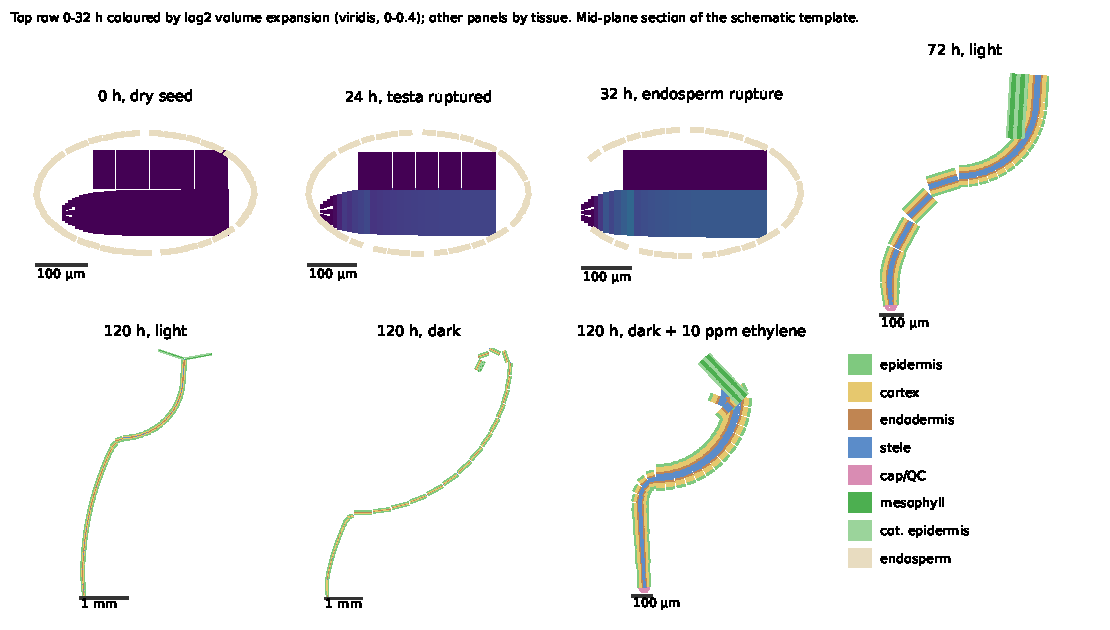
\includegraphics[width=\linewidth]{../figures/fig1_seed_through_time.pdf}
\caption{The twin through time: mid-plane sections of the schematic cellular seed. Germination panels are coloured by cell volume
expansion; seedling panels by tissue. At 120~h, compare light, darkness and darkness with 10~ppm ethylene (triple response).}
\label{fig:seed}
\end{figure}

\subsection{Calibrated germination}
The seed, its cells and their growth are shown through time in Fig.~\ref{fig:seed}.
The calibrated seed ruptures its testa at \FitTR{}~h and its endosperm at \FitER{}~h (observed: 20--31~h and 31--45~h for Col-0
\citep{dekkers2013}; 28--32~h for the endosperm-rupture phase \citep{bassel2014}). Lower-hypocotyl expansion begins at \FitOnset{}~h
(observed 16--22~h) and relative expansion peaks at cortical cell \FitPeak{} (observed $\approx$8) (Fig.~\ref{fig:cal}). ABA falls to
\AbaRatio{} of its initial level by 12~h (observed 0.30 \citep{okamoto2006}), and the endosperm cap ruptures at \FitCap{} of its
initial strength (observed $\approx$0.6 in \emph{Lepidium} \citep{linkies2010}). In seedlings, cotyledons emerge at \SfCotOut{}~h and
open at \SfCotOpen{}~h (observed 60 and 72~h \citep{boyes2001}). Peak hypocotyl growth is \SfHypDark{} and \SfHypLight{}~mm\,d$^{-1}$
in darkness and light (observed 5.96 and 1.11 \citep{alimchandani2026}). Seedling ethylene emission is \SfEth{}~pL\,h$^{-1}$
(observed 0.26--0.53 \citep{heslopharrison2024}). Root elongation at 120~h, \SfRoot{}~$\mu$m\,h$^{-1}$, falls below the rate
extrapolated from day-6 kinematics, a discrepancy we report rather than fit away.

\begin{figure}[t]
\centering
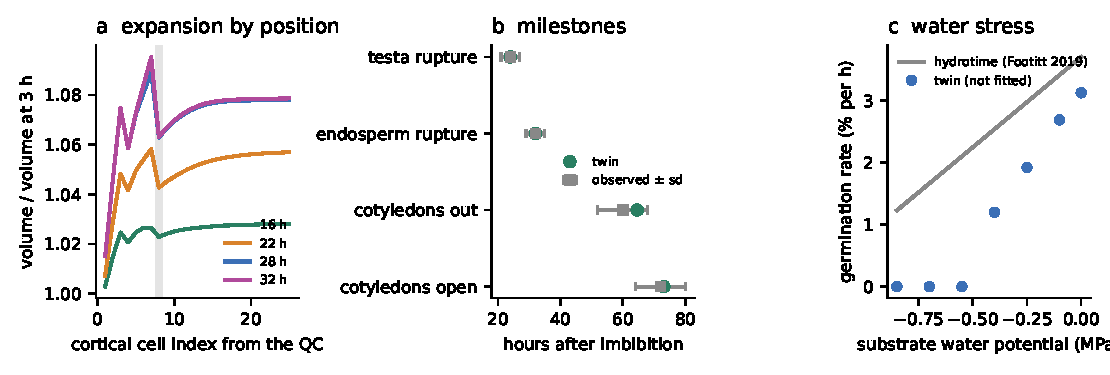
\includegraphics[width=\linewidth]{../figures/fig2_calibration.pdf}
\caption{Calibration and an out-of-sample test. (a) Cortical cell volume relative to 3~h by position from the quiescent centre; grey:
observed peak position (Bassel et al.\ 2014). (b) Simulated milestones against observed values. (c) Germination rate against substrate
water potential: twin (points, not fitted to these data) and the hydrotime model of Footitt et al.\ 2019 (line).}
\label{fig:cal}
\end{figure}

\subsection{Out-of-sample checks}
Neither check below was used in calibration.

\emph{Population spread.} We drew each seed's base water potential from the measured between-seed spread
($\sigma_{\psi_b}$ = 0.222~MPa \citep{footitt2019}). \PopGroundGmax{}\% of \PopGroundN{} seeds then rupture the endosperm, with
t$_{50}$ = \PopGroundTfifty{}~h and a 16--84\% span of \PopGroundSpread{}~h. For the same seeds, hydrotime theory gives t$_{50}$ =
\PopGroundHydTfifty{}~h and a span of \PopGroundHydSpread{}~h, and Col-0 seed lots complete endosperm rupture between 31 and 45~h
\citep{dekkers2013}. The twin therefore turns a given spread of $\psi_b$ into a wider spread of germination times than hydrotime does.

\emph{Water stress.} Lowering the substrate water potential slows the twin's mean seed considerably more than hydrotime
predicts:

\begin{center}
\begin{tabular}{lccc}
\toprule
 & 0~MPa & $-0.25$~MPa & $-0.4$~MPa \\
\midrule
Twin (h) & \HydZeroModel{} & \HydQuarterModel{} & \HydFortyModel{} \\
Hydrotime (h) & \HydZeroTheory{} & \HydQuarterTheory{} & \HydFortyTheory{} \\
\bottomrule
\end{tabular}
\end{center}

\noindent At $-0.55$~MPa and below the twin does not germinate at all (\HydFiftyFiveModel{}~h), whereas hydrotime predicts
\HydFiftyFiveTheory{}~h at $-0.55$~MPa and \HydEightyFiveTheory{}~h at $-0.85$~MPa (at 15~$^\circ$C). The twin's effective base water
potential is thus near $-0.5$~MPa rather than $-1.27$~MPa. The most likely cause is the \emph{assumed} decline of the imbibition plateau
with water potential: it also scales metabolic activation and the GA signal, adding to the hydrotime-linked turgor. We report this
mismatch rather than refit that parameter, which would turn the check into an in-sample fit.

\subsection{Hardware environments}
In every hardware preset, embryo-surface O$_2$ falls well below headspace O$_2$ (Fig.~\ref{fig:hw}). Headspace depletion is
smaller: even in sealed BRIC-PDFU, headspace O$_2$ falls from \BricHsStart{} to \BricHsEnd{}~kPa over 120~h as the seedlings grow. In sealed BRIC-PDFU the minimum embryo-surface pO$_2$ is \BricOSurf{}~kPa against \GroundOSurf{}~kPa on the
ground, and \BricHypoFrac{}\% of embryo cells are hypoxic (pO$_2$ $<$ 1~kPa) at 24~h against \GroundHypoFrac{}\%. With the proxy
tissue diffusivity and respiration rate, the stele core of the axis is anoxic in every environment, so the environment changes the
size of the hypoxic region rather than whether there is one. The resistance that matters is the seed's own coat and
tissue. Sealed hardware accumulates seedling ethylene to a peak of \BricEthHs{}~ppb in BRIC-PDFU, below the lowest concentration
(0.125~ppm) that promoted germination of dormant Col-0 seeds \citep{wang2018}; the twin therefore predicts no ethylene triple response from seedling emission alone, consistent with the curated BRIC-PDFU record, which notes that Millar et al.~\citep{millar2011} saw no ethylene triple
response in sealed PDFUs compared with open dishes. A cabin-air exchange at the
Mir-measured 1.1--1.7~ppm would change this: the twin's dark hypocotyl at 10~ppm reaches \EthTenHyp{}~$\mu$m against \GroundDarkHyp{}~$\mu$m in air.
At the GBC1 seed bed the pump-driven air speed is \GbcULow--\GbcUHigh{}~mm\,s$^{-1}$ (0.25--0.85~L\,min$^{-1}$), giving
$\mathrm{Sh}\approx$\GbcSh{}: the pump renews the headspace but does not ventilate the seed boundary layer.

\begin{figure}[t]
\centering
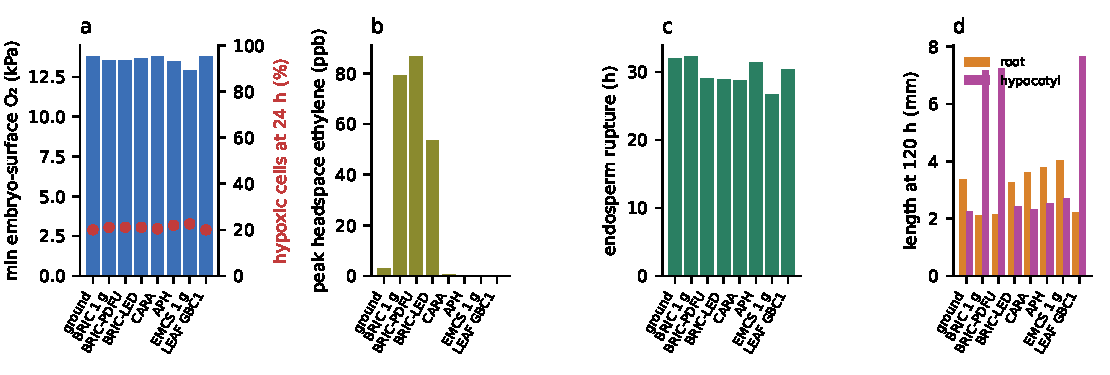
\includegraphics[width=\linewidth]{../figures/fig3_hardware.pdf}
\caption{Hardware environments. (a) Minimum embryo-surface O$_2$ (bars) and percentage of hypoxic embryo cells at 24~h (points). (b) Peak headspace ethylene.
(c) Endosperm rupture time. (d) Root and hypocotyl length at 120~h.}
\label{fig:hw}
\end{figure}

\subsection{Gravity, atmosphere and radiation}
On the EMCS centrifuge preset, root tips turn toward gravity at a rate scaled by the gravity--auxin-asymmetry relation and do not bend
at 0\,g (Fig.~\ref{fig:env}a). The exploration atmosphere (56.5~kPa, 34\% O$_2$) gives a pO$_2$ about 10\% below sea level and raises gas
diffusivity. Because the resistance lies in water and tissue rather than air, faster gas diffusion barely helps: embryo-surface
O$_2$ is \ExploOSurf{}~kPa (sea level \GroundOSurf{}~kPa) and endosperm rupture moves from \GroundER{} to \ExploER{}~h. Uncompensated
air at 56.5~kPa lowers embryo-surface O$_2$ to \CounterOSurf{}~kPa and delays rupture to \CounterER{}~h; 10\% and 5\% O$_2$ at
1~atm delay it to \HypoTenER{} and \HypoFiveER{}~h, consistent with the O$_2$ requirement of germinating Brassicaceae seeds
\citep{park2016}. Radiation has, by construction, no effect unless the hypothesis couplings are switched on (Fig.~\ref{fig:env}c): with all three set
to 1, the solar-particle-event scenario shortens the 120~h root from \SpeRoot{} to \SpeHypRoot{}~$\mu$m. Seeds at 0\,g rupture the
endosperm earlier than at 1\,g in the same hardware (BRIC-PDFU \BricER{} vs \BricOneGER{}~h; EMCS \EmcsZeroER{} vs
\EmcsOneER{}~h) because the \emph{assumed} larger wetted fraction at 0\,g speeds imbibition; the size of this effect rests on assumed
values.

\begin{figure}[t]
\centering
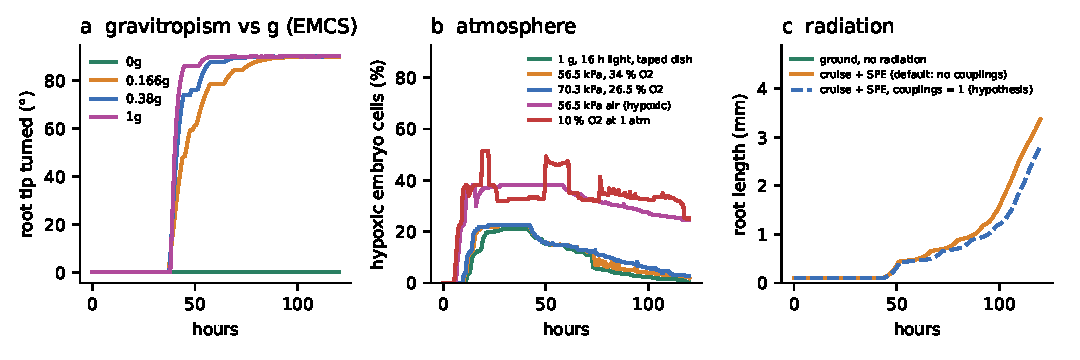
\includegraphics[width=\linewidth]{../figures/fig4_gravity_atmosphere_radiation.pdf}
\caption{(a) Root tip angle on the EMCS preset at four gravity levels. (b) Percentage of hypoxic embryo cells under exploration and hypoxic atmospheres.
(c) Root length under a solar particle event without (solid) and with (dashed) the radiation hypothesis couplings.}
\label{fig:env}
\end{figure}

\subsection{Simulated exposure and observed cell-type signatures}
At 24~h in sealed BRIC-PDFU, the simulated O$_2$ deficit of each atlas cell type and the observed low-oxygen enrichment of that cell
type in the decoder have Spearman $\rho$ = \RhoBric{} ($p$ = \PvalBric{}, $n$ = \NClustBric{} clusters; Fig.~\ref{fig:dec}). This is a
weak test --- the decoder scores marker programmes, not exposure --- but it is the comparison the two tools are designed to support. The ranking of simulated deficits is the same in every scenario
(it is set by the radial geometry), so the agreement tests the model's radial structure, not its response to the environment.

\begin{figure}[t]
\centering
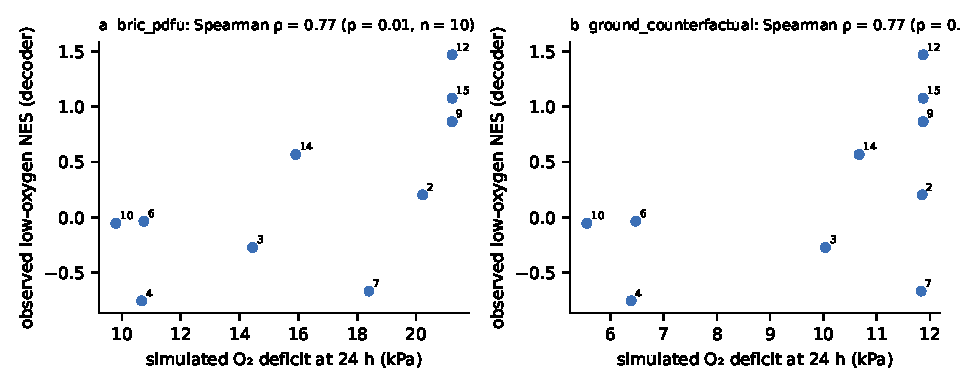
\includegraphics[width=0.85\linewidth]{../figures/fig5_exposure_vs_decoder.pdf}
\caption{Simulated O$_2$ deficit at 24~h per atlas cell type against the observed low-oxygen NES of that cell type in the decoder.}
\label{fig:dec}
\end{figure}

\section{Discussion}
The twin turns the Bassel et al.\ embryo-growth mechanism into a seed in an environment. Three predictions follow that flight data can
test. First, embryo hypoxia in flight hardware is set by the seed coat and tissue, so it should differ little between sealed and
ventilated hardware during germination. Second, at seed scale gravity acts through water films and, after protrusion, tropisms --- not
through the air boundary layer, which is at the still-air limit in sealed dishes and barely ventilated even in the pumped GBC1. Third,
seedling ethylene alone does not reach response levels in sealed dishes; cabin ethylene does.

\paragraph{Limitations.} The geometry is schematic. \TierAssumed{} parameters remain assumed. Several sources are proxies:
\emph{Brassica napus} tissue diffusivity, \emph{Lepidium} cap mechanics, and tomato and apple ACC oxidase. The calibration is not
identifiable. The Topham et al.\ and Bassel et al.\ supplementary equations could not be retrieved, and the hormone core uses the fully
published Abley et al.\ model. Radiation-to-hormone couplings are hypotheses.

\paragraph{Data and code availability.} Code (MIT), ledger, presets, calibration targets, results tables and figures:
\url{https://github.com/dr-richard-barker/deepspace-seed-twin}; live tool: \url{https://dr-richard-barker.github.io/deepspace-seed-twin/}.
Zenodo archive: \todo{DOI after deposit}.

\paragraph{Author contributions, funding, competing interests.} \todo{to be provided by the author}

\bibliographystyle{unsrtnat}
\bibliography{references}
\end{document}
